\documentclass[10pt, a4paper,openany]{article}
\usepackage[italian]{babel}
\usepackage[T1]{fontenc}
\usepackage[table]{xcolor}
\usepackage{float}
\restylefloat{table,figure}
\usepackage{graphicx}	
\usepackage[utf8]{inputenc}
\usepackage{amsmath}
\usepackage{fancyhdr}
\usepackage{geometry}
\usepackage{url}
\usepackage[ruled,vlined]{algorithm2e}
\geometry{a4paper,top=2cm,bottom=2cm,left=3cm,right=3cm,%
	heightrounded,bindingoffset=5mm}
\usepackage{amssymb}
\usepackage{amsthm}


\begin{document}

\begin{center}
\huge\textbf{YouTube al tempo del Covid-19}

Un'analisi dei video in tendenza
\end{center}

\begin{center}
Gabriele Celeri, Federico Luzzi,  Marco Peracchi, Christian Uccheddu
\end{center}

\hrule
\vspace{0.2cm}
\begin{center}\textbf{Introduzione e obiettivi}\end{center} 
Il Covid-19 ha avuto un impatto notevole sulle vite di tutti noi negli ultimi mesi. L'obiettivo di questo lavoro è capire se i video di YouTube siano stati influenzati dalla presenza di questo virus che ha costretto gran parte della popolazione mondiale nelle proprie case. 
Per capire questo impatto abbiamo deciso di confrontare gli andamenti dei video in tendenza nel periodo Dicembre-Gennaio rispetto a quelli nel periodo Marzo-Maggio in modo da poter vedere se i contenuti dei video e le tipologie di questi siano cambiate. 
Avendo questo tipo di dati a disposizione ci siamo inoltre chiesti se le notizie, soprattutto negative, derivanti dal numero di contagiati, influenzasse la fruizione di video riguardanti il Covid-19.
\\\\ \begin{small}
	\textit{Keyword: Covid-19, YouTube}
\end{small}
\vspace{0.2cm}
\hrule

\subsection*{Scelta degli strumenti (DA RISCRIVERE)}
La prima domanda che ci siamo posti riguardo al progetto è stata: "Quali sono le "V" su cui focalizzare la nostra attenzione?".
Dopo qualche indagine preliminare abbiamo deciso che che ci saremmo concentrati su "Volume" e su "Velocity", perché i nostri dati venivano raccolti in tempo reale dalle API di Youtube e la quantità di dati aumenta costantemente con l'aumentare del tempo di presa dati.

Per gestire il flusso di dati ci siamo affidati al software Kafka, permettendoci così di poter disaccoppiare la fase di lettura dei dati dalla fase di  raccolta. Uno script python (\textit{scraper\_producer.py}) si occupava del producer, continuando ad effettuare richieste alle API di youtube, mentre lo script consumer (\textit{scraper\_consumer.py}) si occupava di leggere i file memorizzati nel topic di kafka, e successivamente di immagazzinarli in un database MongoDB in formato JSON. La scelta di MongoDB è stata dettata dalla sorgente dei dati, che venivano forniti in formato documentale.
\section*{Raccolta dati}
La raccolta dati è basata su due fonti principali: YouTube e [fonte/i covid-19].
\subsection*{Youtube API}
I video in tendenza su youtube variano ogni 15 minuti circa (fonte: \url{https://support.google.com/youtube/answer/7239739?hl=it}) anche se non per forza e solitamente vi è solo una manciata di video che entra/esce dalle tendenze. Per la raccolta di questi dati ci siamo basati sulle funzioni API messe a disposizione da youtube per poter raccogliere i video in tendenza in un dato momento. Le chiavi di richiesta gratuite fornite da Google developer però ci permettono di effettuare una quantità limitata di richieste. 
\\
Abbiamo effettuato sostanzialmente due differenti \textbf{sessioni} di scraping, con metodi leggermente differenti, dovuti allo scopo che ci eravamo prefissati: 
\begin{enumerate}
	\item dal 23 dicembre 2019 al 5 gennaio 2020 (raccolta ogni 30 minuti)
	\item dal 18 marzo 2020 al 6 maggio 2020 (raccolta ogni 6 ore)
\end{enumerate}
Abbiamo deciso di raccogliere dati delle tendenze dei seguenti paesi:

Italia, USA, Regno Unito, India, Germania, Canada, Francia, Corea del sud, Russia, Giappone, Brasile, Messico\\

\subsection*{Prima sessione}
Inizialmente pensavamo di utilizzare i dati per analizzare come, in generale, un video riesce ad arrivare nelle tendenze di youtube e in base a questo fatto analizzare il suo comportamento per quanto riguarda visualizzazioni, likes, dislikes, ecc. La raccolta in questa sessione viene effettuata con lo script \textit{scraper\_timed.py} che sostanzialmente esegue questi passaggi:\\
\\
\begin{algorithm}[H]
	\KwData{country - insieme dei paesi prescelti; videos - insieme di video scaricati da un determinato paese}
	\nl \For{every 30 minutes} {
	\nl \ForEach{country}
	{
		\nl videos = APIrequest(max(50 video), country)\\
		\nl \While {video in tendenza non finiti}
		{
			\nl videos += APIrequest(max(50 video), country) \\
		}
		\nl videos\_fix = arrangeData(videos)\\ 
		\nl saveToCsv(videos\_fix) \\
		\nl videos = $\emptyset$
	}
	}
	\caption{Scraping youtube $\rightarrow$ csv}
\end{algorithm}

%Alternativa per scrivere l'algoritmo
%\begin{enumerate}
%	\item Per ogni paese prescelto
%	\item API request sulle tendenze del momento $\rightarrow$ download di page da 50 video [formato json]
%	\item ripeti 2. finchè scarica tutti i video
%	\item copio le informazioni formattate in formato csv (vedi dopo) 
%	\item ripeti da 2. per ogni paese
%	\item attendi 30 minuti (scheduler)
%	\item ripeti da 1.
%\end{enumerate}
\underline{Nota}: per ogni API request al massimo possiamo scaricare 50 video e ogni paese a un numero diverso di video in tendenza (solitamente 150-200).

In questa sessione abbiamo pensato di salvare i dati in formato \textit{csv}
modo tale che siano facilmente manipolabili. Segue lo schema logico con cui li abbiamo immagazzinati:
\begin{table}[H]
	\centering
	\begin{tabular}{l|l}
		\textbf{Attributo} & \textbf{Descrizione} \\
		\hline
		\textbf{timestamp} & data, ora e minuto della nostra rilevazione \\\hline
		\textbf{video\_id} & identificativo unico del video\\\hline
		\textbf{title} & nome del video per esteso\\\hline
		\textbf{publishedAt} & data di pubblicazione\\\hline
		\textbf{channelId} & identificativo unico del canale che ha pubblicato il video\\\hline
		\textbf{channelTitle} & nome del canale per esteso\\\hline
		\textbf{categoryId} & identificativo unico della categoria\\\hline
		\textbf{trending\_date} & data in cui il video è in tendenza\\\hline
		\textbf{tags} & stringa dei tag usati separati dal carattere "|"\\\hline
		\textbf{view\_count} & numero di visualizzazioni\\\hline
		\textbf{likes} & numero di like (mi piace)\\\hline
		\textbf{dislikes} & numero di dislike (non mi piace)\\\hline
		\textbf{comment\_count} & numero di commenti sotto il video\\\hline
		\textbf{thumbnail\_link} & url all'immagine di copertina del video\\\hline
		\textbf{comments\_disabled} & booleano che dichiara se i commenti sono disabilitati\\\hline
		\textbf{ratings\_disabled} & booleano che dichiara se i like/dislike sono disabilitati\\\hline
		\textbf{description} & descrizione del video\\
		\hline
	\end{tabular}
	\caption{schema degli attributi dei dati csv}
\end{table}

I dati così raccolti sono salvati nella cartella [INSERIRE NOME CARTELLA]

\subsection*{Seconda sessione}

Per la seconda sessione di raccolta, in cui abbiamo deciso di concentrarci sugli effetti che l'epidemia del nuovo virus Covid-19, abbiamo adottato un approccio diverso. Innanzitutto abbiamo deciso di immagazzinare i dati in un database mongoDB nativamente. Pertanto oltre a costruire una pipeline di raccolta che salva i dati direttamente su mongoDB abbiamo deciso parallelamente di immagazzinarli in formato \textit{json}. 

Seconda considerazione è stata data la bassa variabilità dei video raccogliendo i dati ogni 30 minuti, vista nella precedente sessione, abbiamo deciso di effettuare lo scraping ogni 6 ore, in modo da avere 4 rilevazioni durante una giornata. 

A scopo didattico abbiamo inoltre deciso di implementare una piccola pipeline Kafka in cui dividiamo la fase di raccolta dati (\textit{scraper\_producer.py}) e la fase di immagazzinamento (\textit{scraper\_consumer.py}). 

\begin{figure}[H]
	\centering
	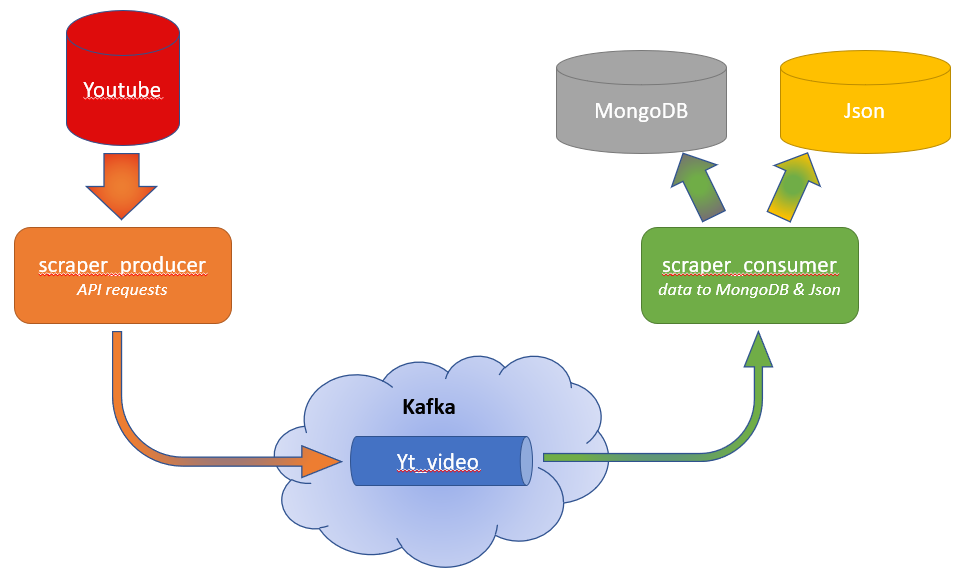
\includegraphics[width=0.8\linewidth]{pics/pipeline.png}
	\caption{pipeline di raccolta dati - seconda sessione}
\end{figure}

Di seguito il dettaglio della computazione dei 2 script:

\begin{algorithm}[H]
	\KwData{country - insieme dei paesi prescelti; videos - insieme di video scaricati da un determinato paese; KafkaProducer(data, channel) - sends data to channel kafka}
	\nl \For{every 6 hours} {
		\nl \ForEach{country}
		{
			\nl videos = APIrequest(max(50 video), country)\\
			\nl KafkaProducer(videos, yt\_video) \\ 
			\nl \While {video in tendenza non finiti}
			{
				\nl videos = APIrequest(max(50 video), country) \\
				\nl KafkaProducer(videos, yt\_video) \\
			}
		}
	}
	\caption{scraper producer}
\end{algorithm}

\begin{algorithm}[H]
	\KwData{KafkaConsumer(channel) - receives data from channel kafka}
	\nl \While{loop} {
		\nl \If{KafkaConsumer(yt\_video) $\ne \emptyset$}
		{
			\nl videos = KafkaConsumer(yt\_video)\\
			\nl videos\_fix = arrangeData(videos)\\ 
			\nl saveToJson(videos\_fix)\\
			\nl saveToMongoDB(videos\_fix)
		}
	}
	\caption{scraper consumer}
\end{algorithm}
I dati così raccolti sono stati salvati in formato json nella cartella [INSERIRE NOME CARTELLA].

\underline{Nota}: abbiamo scelto di salvare i dati in formato Json in modo che fosse facile caricarli in un nuovo server mongoDB e renderli più trasportabili. Per il caricamento vedi lo script: \textit{json\_to\_mongo.py}

Lo schema logico dei documenti json è sostanzialmente lo stesso di quello dei csv visto precedentemente in \textit{Tabella 1} ma con due variazioni:
\begin{itemize}
	\item \textbf{tags} immagazzinati come array di stringhe
	
	Ad esempio:
	
	tags: ["covid-19", "quarantena"]
	\item informazioni relative ai likes, dislikes, view\_count e comment\_count innestati in un oggetto \textbf{statistics}
	
	Ad esempio:
	
	statistics: \{view\_count: 14235,
				likes: 513,
				dislikes: 34,
				comment\_count: 254
				\}
\end{itemize}
\subsection*{Dati Covid-19}
Qua dobbiamo scrivere come/dove abbiamo preso i dati covid

  
\subsection*{Qualità dati}
Avendo una grande mole di dati ci siamo dovuti anche occupare di verificare la pulizia o meno del nostro dataset. Per prima cosa abbiamo notato che non c'era presenza di Missing Values, questo è stato di per sé una grande fortuna poiché di solito il Missing Replacement è una operazione molto lunga.  Ci sono state però due problematiche principali che abbiamo dovuto affrontare:
\begin{itemize}
	\item Ridondanza: Questo problema è nato dal fatto che i trending di Youtube sono stati presi ogni mezz'ora, con il risultato di avere molti dati simili riguardanti le stesse fasce della giornata. 
	\item Buchi: Questo problema è nato dal fatto che Google non permette di avanzare troppe richieste per la presa dati nella stessa giornata, per arginare questo problema abbiamo utilizzato 3 chiavi diverse con cui mandare le richieste a Google in modo tale da coprire la maggior parte della giornata. Ci sono stati però dei punti in cui la presa dati non è riuscita. Il metodo che abbiamo utilizzato per riempire quei buchi è stato quello di duplicare i dati della presa dati precedente. Questo metodo è stato possibile poiché la presa dati è stat effettuata in intervalli di tempo in cui i dati non vengono modificati significativamente.
	
\end{itemize}

\subsection*{Integrazione dati}
	Per poter rispondere alle nostre domande di ricerca abbiamo dovuto effettuare un'integrazione tra i dati dei video di Youtube e i dati relativi ai contagi giornalieri di covid-19. Il merge l'abbiamo effettuato prima del loro caricamento su MongoDB. Lo script che implementa la nostra integrazione è \textit{merge\_to\_mongo.py}. 
	
	Sostanzialmente applichiamo un'\textbf{integrazione temporale} considerando, per ciascun video, il \textbf{timestamp} della rilevazione e il paese in cui il video è presente (\textbf{country\_name}). Ricerchiamo il corrispettivo (timestamp, country\_name) nella base dati covid e generiamo un nuovo documento con tutte le informazioni del video di Youtube aggiungendo un sotto documento \textit{covid} con tutti i dati relativi ai contagi avvenuti quel giorno in quello stato. A questo punto i documenti vengono caricati su MongoDB.
	
	Un problema riscontrato durante l'integrazione è stato che la rilevazione viene effettuata con il fuso orario di Greenwich GMT, però ciascun paese ha uno o più fusi orari differenti. Pertanto abbiamo corretto i timestamp in base al fuso orario della capitale di ciascun paese. Nel dettaglio visualizzare il file \textit{country\_name.json}.
	
	L'operazione di integrazione complessivamente richiede:
	\begin{itemize}
		\item senza sharding: 1419 s (23,6 min circa)
		\item con sharding: 1431 s (24 min circa)
	\end{itemize}
\subsection*{Espressione regolare}
	Per poter distinguere quali video possono essere considerati legati al covid-19 o meno, abbiamo definito la seguente espressione regolare:
	\begin{figure}[H]
		\centering
		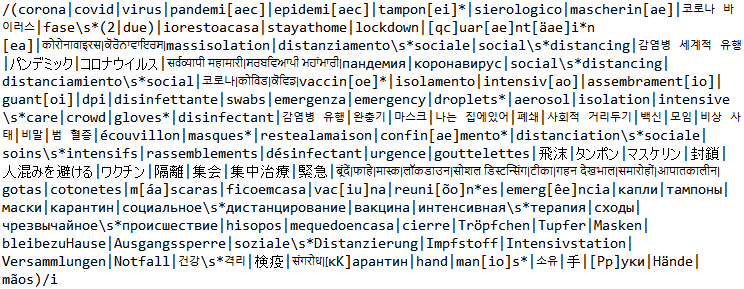
\includegraphics[width=0.95\linewidth]{pics/er.png}
	\end{figure}

	Abbiamo cercato di includere tutte le parole legate al contesto del Covid-19 e la loro traduzione in tutte le lingue dei paesi del nostro studio.
	
	Questa espressione regolare l'abbiamo applicata sia analizzando i titoli dei video, sia analizzando i tags scelti per descrivere il video. L'applicazione è avvenuta tramite le seguenti query:
	\begin{enumerate}
		\item setting tutti video come non covid (sia per titolo che per tags):
		
			db.video\_merge.update(\{\},\{\$set : \{covid\_tags : false, covid\_title : false\}\},\{multi : true\})
		
		\item setting true tutti i video che hanno almeno un tag che rispetta l'espressione regolare (REGEX):
		
			db.video\_merge.update(\{tags : \{\$in : [REGEX]\}\}, \{\$set : \{covid\_tags: true\}\}, \{multi : true\})
		
		\item setting true tutti i video il cui titolo rispetta l'espressione regolare (REGEX):
		
			db.video\_merge.update(\{title : \{\$in : [REGEX]\}\}, \{\$set : \{covid\_title: true\}\}, \{multi : true\})
	\end{enumerate}

\subsection*{Scalabilità dell'algoritmo}

Visto che una delle V che abbiamo deciso di usare concernenti i Big Data è stata quella relativa al volume dobbiamo occuparci di vedere come si comporta la nostra elaborazione dati con volumi di dati sempre crescenti. Abbiamo deciso di implementare lo \textbf{Sharding} su MongoDB. In particolare, abbiamo deciso di costruire 3 shard replica group formati da 3 repliche dello shard in modo da garantire la ridondanza nel caso di guasti e la frammentazione per rendere più efficienti le query. La chiave di sharding scelta è quella del campo "\textbf{country\_name}" perché le query per rispondere alle nostre domande vengono fatte sul singolo paese. Questo approccio è stato pensato anche nell'ottica di dividere la grande mole di dati in server disposti in ciascun paese. 

Segue lo schema logico applicato:
\begin{figure}[H]
	\centering
	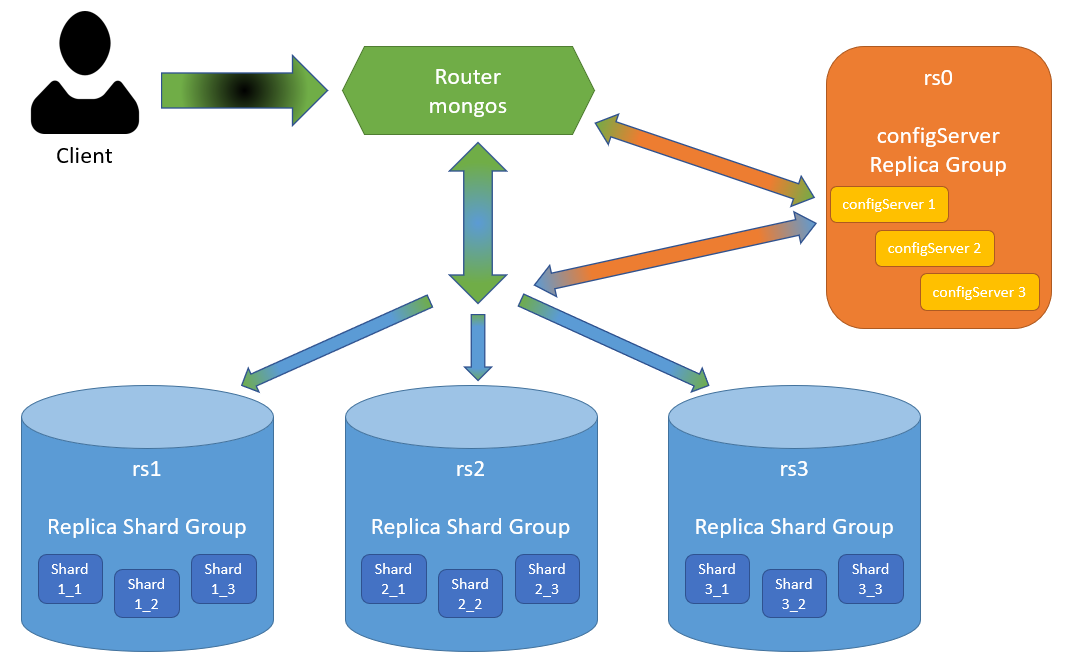
\includegraphics[width=0.8\linewidth]{pics/sharding.png}
	\caption{Pipeline sharding}
\end{figure}

QUERY ANALISI:


%Per farlo ci occupiamo di effettuare la nostra analisi su partizionamenti sempre maggiori del nostro dataset e registriamo il tempo di esecuzione del nostro programma, effettuiamo poi una semplice regressione per vedere di che tipo di crescita stiamo parlando, ovviamente più la crescita è minore più il nostro algoritmo scala bene per volumi di dati maggiori. Presentiamo di seguito la registrazione dei tempi rispetto al partizionamento dei dati. 

%\begin{figure}[H]
%	\centering
%	\includegraphics[height=0.3 \linewidth]{pict/times.png}
%	\caption{Crescita del tempo di esecuzione rispetto all'aumentare del partizionamento.}
%\end{figure}

\section*{Visualizzazione}
Per la scelta delle visualizzazione abbiamo dovuto pensare per prima cosa a delle domande di ricerca a cui rispondere. Le domande che ci siamo posti sono le seguenti:
\begin{itemize}
	\item Variazione della tipologia di video in tendenza da periodo pre covid-19 a periodo covid-19
	\item È vero che la fruizione di video su Youtube riguardanti i contagi di Covid-19 segue l'andamento dei dati sull'epidemia?
\end{itemize}

\subsection*{Scelta features}
Per rispondere in modo coerente alle nostre domande di ricerca abbiamo deciso di concentrarsi sulle seguenti features del nostro dataset.
\begin{itemize}
	\item View Count
	\item Covid Title
	\item Covid Tags
	\item Trending Date
	\item Title
	\item Cases New
\end{itemize}

\subsection*{Scelta della visualizzazione}

Per rispondere alle due domande di ricerca che ci siamo posti abbiamo deciso di utilizzare due infografiche diverse. La scelta di utilizzare due infografiche diverse è stata data dal fatto che le due domande sono incompatibili tra loro e quindi sarebbe stato impossibile utilizzarne una unica.

\paragraph{Prima infografica} La prima infografica consiste nella combinazione di due diverse visualizzazioni:
\begin{itemize}
	\item La prima visualizzazione è costituita da un istogramma temporale che rappresenta il numero video entrato in tendenza ogni giorno.
	\item La seconda riguarda è costituita da un bubble chart e riguarda il numero di video per ogni categoria entrato in tendenza quel giorno.
\end{itemize}
La combinazione di queste due visualizzazioni permette di capire se il contenuto dei video entrati in tendenza nel periodo pre Covid-19 e post Covid-19 differiscano significativamente. Per farlo è sufficiente selezionare due giorni contemporaneamente e vedere il cambiamento nelle bolle. L'esplorazione di questa infografica avviene per step in modo da avvicinare l'utente piano piano a tutte le informazioni che questa infografica può offrire. Di seguito una visione sommaria dell'infografica comprensiva dei contesti:
\begin{figure}[H]
	\centering
	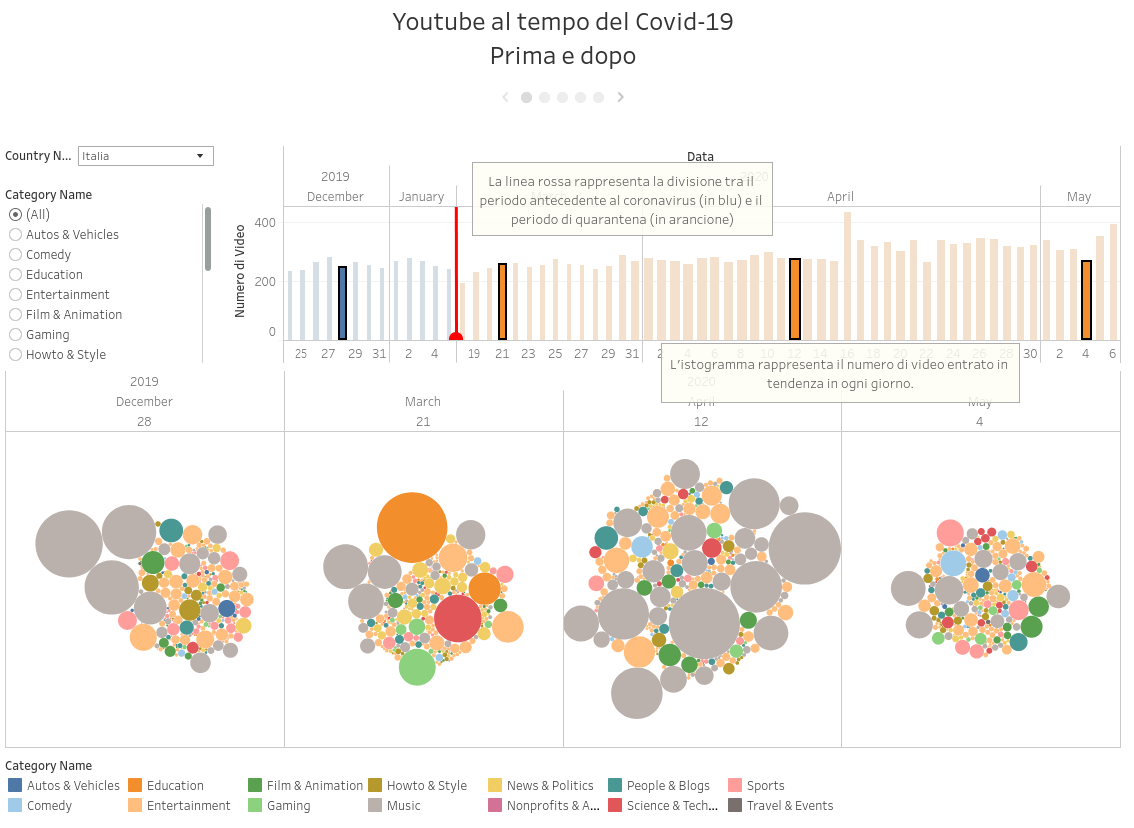
\includegraphics[height=0.5 \linewidth]{pics/prima_infografica.png}
	\caption{Prima infografica.}
\end{figure}

\paragraph{Seconda infografica} Per quanto riguarda la risposta alla seconda domanda di ricerca abbiamo deciso di utilizzare una infografica composta da due visualizzazioni. In particolare:
\begin{itemize}
	\item La prima visualizzazione è un misto tra un bar chart e un line chart temporale. In questa visualizzazione abbiamo fatto risaltare la differenza percentuale tra una rilevazione e la precedente. In particolare il line chart riguarda l'aumento percentuale del numero di video in tendenza relativi al Covid-19 mentre il bar chart riguarda l'aumento percentuale dei nuovi casi di Covid-19 rispetto al giorno precedente. Abbiamo utilizzato questo tipo di grafico in modo da poter vedere se la divulgazione negativa dei dati riguardanti il Covid-19 abbia influito sulla fruizione online dei video riguardanti lo stesso argomento. La scelta di creare due forme diverse per i due andamenti è motivata dal fatto che dai questionari è risultata più apprezzata per riconoscere le due variabili.
	\item La seconda visualizzazione è uno stacked bar chart che rappresenta il numero di video per categoria che riguardano il Covid-19 che può essere filtrata per giorno semplicemente interagendo con la prima visualizzazione.
\end{itemize}

La combinazione di queste due visualizzazioni consente di rispondere alla seconda domanda di ricerca che ci siamo posti precedentemente. Proponiamo di seguito una visione sommaria dell'infografica comprensiva dei contesti.

\begin{figure}[H]
	\centering
	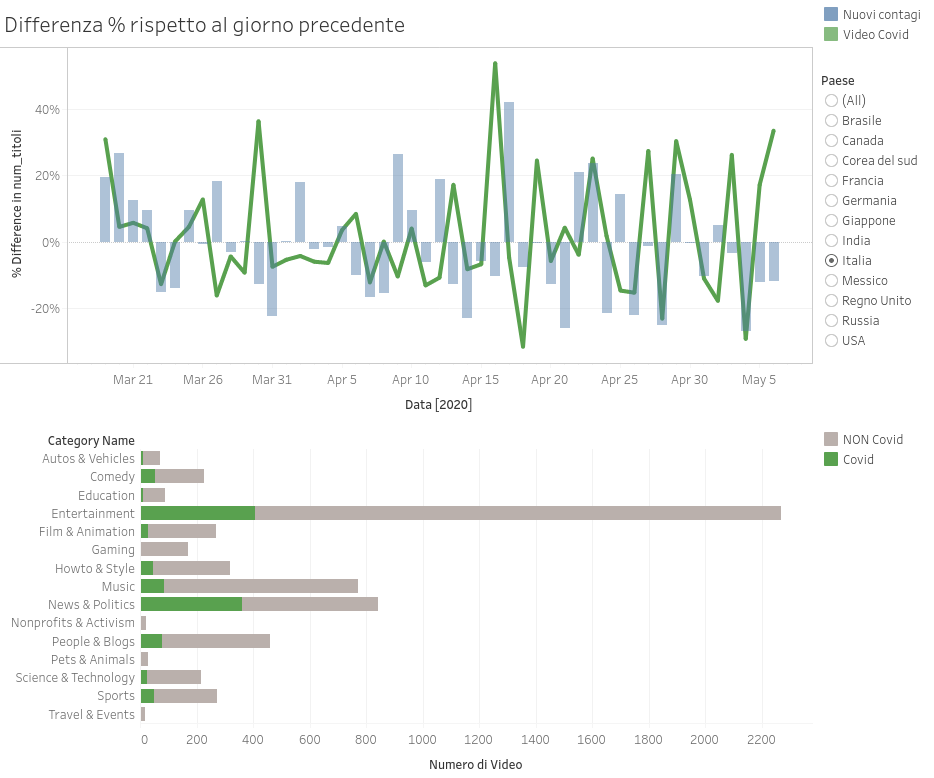
\includegraphics[height=0.5 \linewidth]{pics/seconda_infografica.png}
	\caption{Seconda infografica.}
\end{figure}
\subsection*{Valutazione della qualità}
La valutazione della qualità della nostra infografica si è articolata in tre macro passaggi:

\paragraph{User Test} Durante questa fase ci siamo occupati di sottoporre la nostra infografica a 3 persone lasciando completa libertà di esplorazione. Le varie esplorazioni sono state registrate in modo da far sì che potessero emergere le diverse problematiche di cui non ci siamo accorti in fase di realizzazione delle infografiche. Esponiamo le problematiche emerse durante questa fase di valutazione e le correzioni applicate:

\begin{itemize}
	\item Problema 1: soluzione 1
	\item Problema 2: soluzione 1
	\item Problema 3: soluzione 1
\end{itemize}
\paragraph{Risultati dei task} Durante questa fase ci siamo occupati di sottoporre tre diverse richieste a 24 utenti che dovevano essere soddisfatte esplorando interattivamente la nostra infografica. In particolare i task da risolvere sono stati i seguenti:
\begin{itemize}
	\item Qual'è il video con l'indice di partecipazione più alto in Italia?
	\item Qual'è il video con l'indice di partecipazione più alto tra tutti i paesi?
	\item Che categoria di video dovresti utilizzare se volessi creare contenuti che piacciono in USA?
\end{itemize}Ci siamo occupati di registrare i tempi in cui gli utenti riuscivano a completare questu obiettivi e abbiamo visualizzato questi record nei seguenti violin plot:
%\begin{figure}[H]
%	\centering
%	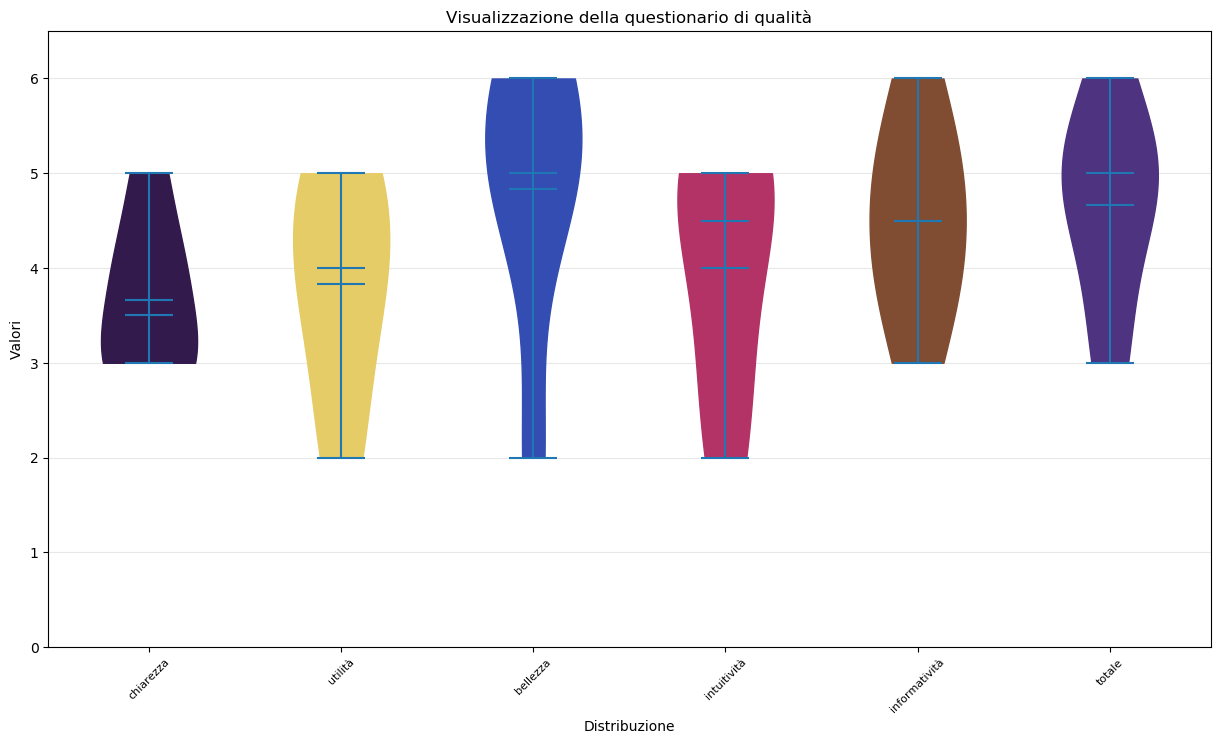
\includegraphics[height=0.3 \linewidth]{pict/violin_plot.png}
%	\caption{Tempi di completamento dei task.}
%\end{figure}
Questa visualizzazione è utile per capire se le nostre infografiche sono troppo dispersive o riescono a centrare gli obietivi facilmente.
\paragraph{Questionari} Per quanto riguarda quest'ultima fase ci siamo occupati di rivolgere un questionario della valutazione della qualità a 24 persone. In particolare il questionario è stato articolato nella seguente maniera:
\begin{itemize}
	\item Come valuti la chiarezza dell' infografica?
	\item Come valuti l'utilità dell'infografica?
	\item Quanto valuti la bellezza dell'infografica?
	\item Come valuti l'intuitività dell'infografica?
	\item Quanto è stata informativa l'infografica?
	\item Come valuti complessivamente l'infografica?
\end{itemize}
Le risposte sono state registrate grazie al tool: Questionari di Google. Una volta registrate le risposte ci siamo occupati di vedere se la valutazione complessiva dell'infografica fosse coerente con una ricostruzione complessiva data dalla regressione con i coefficienti di Cabitza-Locoro.
%\begin{figure}[H]
%	\centering
%	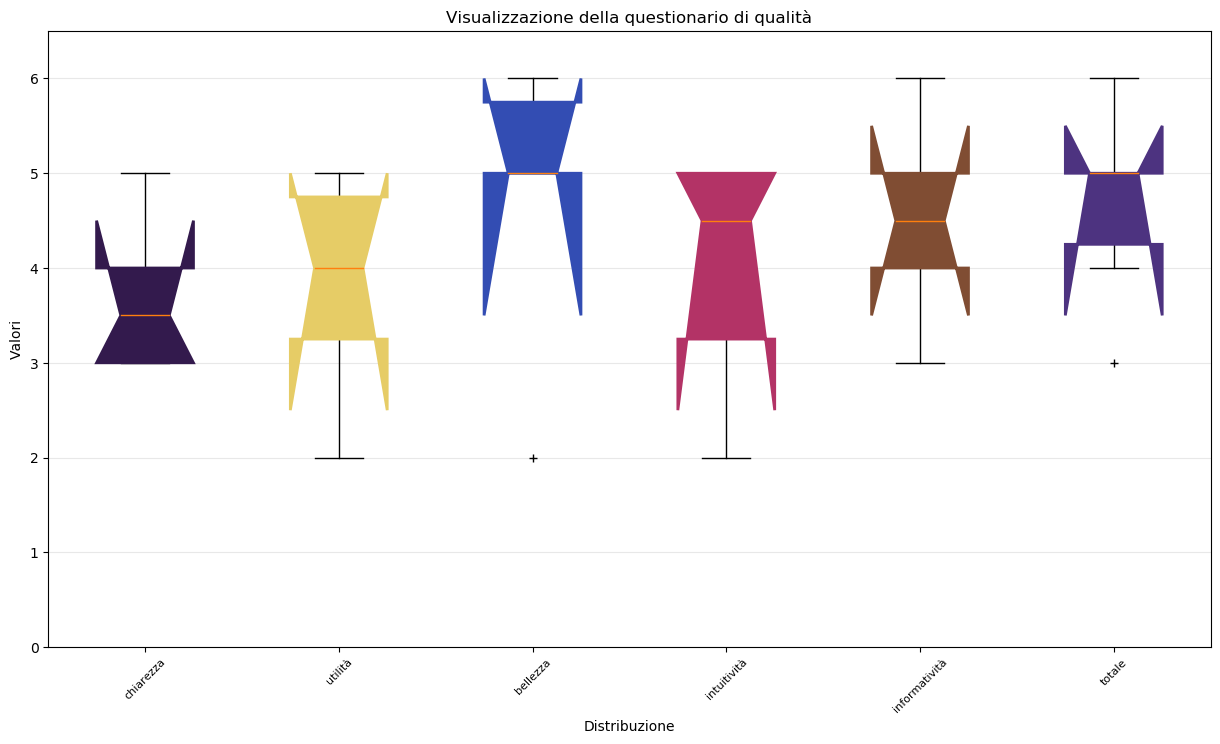
\includegraphics[height=0.3 \linewidth]{pict/box_plot.png}
%	\caption{Dispersione delle risposte del questionario.}
%\end{figure}
E' stato comodo usare un box plot per la registrazione di queste risposte poiché la media è un indicatore di tendenza centrale e non fornisce alcuna informazione sulla distribuzione di questi dati.
Per quanto riguarda invece della coerenza della valutazione complessiva rispetto alla ricostruzione data dai coefficienti abbiamo avuto la seguente distribuzione:
%\begin{figure}[H]
%	\centering
%	\includegraphics[height=0.3 \linewidth]{pict/regressione.png}
%	\caption{$R^{2} = 0.75$.}
%\end{figure}


\end{document}